\documentclass[10pt]{article}

\usepackage{draftcopy}
\usepackage{multirow}
\usepackage{rotating,graphicx}
%\usepackage{wrapfig}
\usepackage{amssymb}
\usepackage{amsmath}
\usepackage{lscape}
\usepackage{times}
\usepackage{color}  % For \textcolor and \color % Ex. : \textcolor{red}{Text colored with} ; {\color{red}Text colored with}
\usepackage{soul}   % For \hl{ highlighted text} ; \sethlcolor{colorname}
%\usepackage[table]{xcolor}
\usepackage{xcolor,colortbl}
\usepackage{capt-of}
\usepackage{textcomp}  % allows \textonehalf,  \textonequarter, or else
%\usepackage{mathcomp}  % make it math compatible

\oddsidemargin =-0.6in
\evensidemargin=-0.6in
%\textwidth=7.6in   % owl
 \textwidth=7.8in % laptop
\textheight=10.2in
% \topmargin=-.25in   % owl
 \topmargin=-1.in    % laptop
\footskip=-.0in

\newcommand{\Bl}{\ensuremath{B_{{low}}}}
\newcommand{\Bh}{\ensuremath{B_{{high}}}}
\newcommand{\Il}{\ensuremath{I_{{low}}}}
\newcommand{\Ih}{\ensuremath{I_{{high}}}}
\newcommand{\Br}{\ensuremath{B\! \rho}}
\newcommand{\CE}{concentration ellipse}
\newcommand{\CES}{CE-$\rm \mathcal{S}$}
\newcommand{\dEE}{\small \ensuremath{\frac{dE}{E}}}
\newcommand{\eg}{\ensuremath{\it e.g.}}
\newcommand{\Ha}{\ensuremath{\mathcal{H}}}
\newcommand{\Sa}{\ensuremath{\mathcal{S}}}
\newcommand{\vs}{\ensuremath{\it vs.}}
\newcommand{\ie}{\ensuremath{\it i.e.}}
\newcommand{\hbrk}{\hfill \break}
\newcommand{\sr}{synchrotron radiation}
\newcommand{\SRl}{SR loss}
\newcommand{\x}{\ensuremath{x}} 
\newcommand{\xp}{\ensuremath{{x'}}}
\newcommand{\z}{\ensuremath{z} }
\newcommand{\zp}{\ensuremath{{z'}}}
\newcommand{\y}{\ensuremath{y} }
\newcommand{\yp}{\ensuremath{{y'}}}
\newcommand{\dl}{\ensuremath{{\delta l}}} 
\newcommand{\dE}{\ensuremath{{\delta E}}}
\newcommand{\X}{\ensuremath{X} }
\newcommand{\Xp}{\ensuremath{{X'}}}
\newcommand{\Z}{\ensuremath{Z} }
\newcommand{\zg}{Zgoubi}
\newcommand{\Zp}{\ensuremath{{Z'}}}
\newcommand{\Y}{\ensuremath{Y} }
\newcommand{\Yp}{\ensuremath{{Y'}}}
\newcommand{\Len}{\ensuremath{l} }
\newcommand{\Mom}{\ensuremath{E}}
\newcommand{\Sx}{\ensuremath{\mathcal{S}_x}}
\newcommand{\Sy}{\ensuremath{\mathcal{S}_y}}
\newcommand{\Sz}{\ensuremath{\mathcal{S}_z}}

\newcommand{\C}{\ensuremath{\mathcal{C}}}
\newcommand{\D}{\ensuremath{\mathcal{D}}}
\newcommand{\HH}{\ensuremath{\mathcal{H}}}
\newcommand{\bHH}{\bar \HH}
\newcommand{\com}{{center of mass}}
\newcommand{\lab}{{laboratory frame}}
\newcommand{\LL}{\ensuremath{\mathcal{L}}}
\newcommand{\rms}{\ensuremath{rms}}
\newcommand{\wrt}{{with respect to}}

\newcommand{\bull}{\ensuremath{\bullet~}}
\newcommand{\cf}{\ensuremath{\textsl{cf.}}}
\newcommand{\bhel}{\ensuremath{\mathbf{^3He^{2+}}}}
\newcommand{\hel}{\ensuremath{\mathrm{^3He^{2+}}}}
\newcommand{\nib}{\noindent \ensuremath{\bullet~}}
\newcommand{\snib}{\noindent {\small \ensuremath{\bullet~}}}
\newcommand{\nid}{\noindent \ensuremath{\diamond~}}
\newcommand{\snid}{\noindent {\small \ensuremath{\diamond~}}}
\newcommand{\nin}{\noindent~}
\newcommand{\no}{\ensuremath{\mathbf{\vec n_0}}}
\newcommand{\MC}{Monte~Carlo}
\newcommand{\p}{\ensuremath{\mathbf{p}}}
\newcommand{\pp}{$\rm p\! \! \uparrow$}

\definecolor{orange}{rgb}{1,0.5,0}
\definecolor{yelloworange}{rgb}{1,.647,0}
\newcommand{\black}{\color{black}}
\newcommand{\red}{\color{red}}
\newcommand{\green}{\color{green}}
\newcommand{\blue}{\color{blue}}
\newcommand{\yo}{\color{yelloworange}}

\newcommand{\referenceA}{\rm  }
\newcommand{\referenceB}{\rm }
\newcommand{\referenceC}{\rm }

\pagestyle{headings}
\markboth{\small  \referenceA ~ ~   \referenceB ~ ~  \referenceC \hfill }
         {\small  \referenceA ~ ~   \referenceB ~ ~  \referenceC \hfill }


\begin{document}

\thispagestyle{empty}

\begin{minipage}{1.\linewidth}
\bf
  \flushright{F. M\'eot}
\vspace{-2ex}
  
  \flushright{BNL C-AD}
\vspace{-2ex}
  
  \flushright{Zgoubi 2019 Workshop, Boulder, CO}
\vspace{-2ex}
  
\flushright{24-29 Aug. 2019} 
\end{minipage}


\vspace{5ex}

\centerline{\LARGE \bf
  An Introduction to ``WIENFILTER'' 
}

~

\centerline{\LARGE \bf
Exercise 2: Using it As a Spin Rotator
}

\vspace{5ex}
\author{
F.~M\'eot
\\
Collider-Accelerator Department, BNL, Upton, NY 11973 \\
}


\section*{Recommended readings}

\smallskip
\nin - Section ``2.7 - Wien filter''  in ../../documentation/eRHICelectronWF.pdf

\smallskip
\nin - Section ``4 - Rotation in dipoles and solenoids''  in ../../documentation/polarizationOfZgoubi.pdf

\smallskip
\nin - Zgoubi Users' Guide, regarding the keywords used in the exercise (WIENFILTER, OBJET/KOPT=2, FIT[2], REBELOTE, etc.). Hint: use the index (last 3 pages of the Guide) to locate the related sections in Part~A and Part~B. 

\smallskip
\nin - During the exercise, it is recommended to keep 2 copies of the guide at hand, with one copy opened at the Index (last 3 pages of the document).

\section*{Keywords we play with in this exercise}

\texttt{WIENFILTER} is used in this exercise (pp.~168 and 306 in the Users' Guide).  B and E are set so to ensure (i)~straight trajectory across the Wien filter,  (ii)~proper spin rotation from initial longitudinal orientation.


\bigskip

\nin
\begin{minipage}{0.6\linewidth}
\section*{Working hypotheses}

- The Wien filter length is $ L$

- Take $ \vec E \parallel \vec Y$ and $ \vec B \parallel \vec Z$ (as sketched to the right)

- E and B fields are taken hard-edge so to allow tight comparison with theory

-  Electron trajectory is straight, so $ E = v \, B$

%\nib In the Wien filter frame, spin rotation is 
%$$ \theta_Z = (1+a\gamma) \dfrac{BL}{B\rho}$$


\paragraph*{Expectations include: } ~ 

- Straight trajectory across the Wien filter (green, in the figure)

- 30$^o$ spin rotation 
$$ \theta_Z =
\underbrace{ (1+a\gamma)\dfrac{BL}{B\rho}}_{\approx 50^o\ from\ \vec B} - \underbrace{ (a\gamma+\dfrac{\gamma}{1+\gamma})\beta^2 \dfrac{BL}{B\rho}}_{\approx 20^o\ from\ \ \vec E} =30^o$$

\end{minipage} \hfill
\begin{minipage}{0.39\linewidth}

  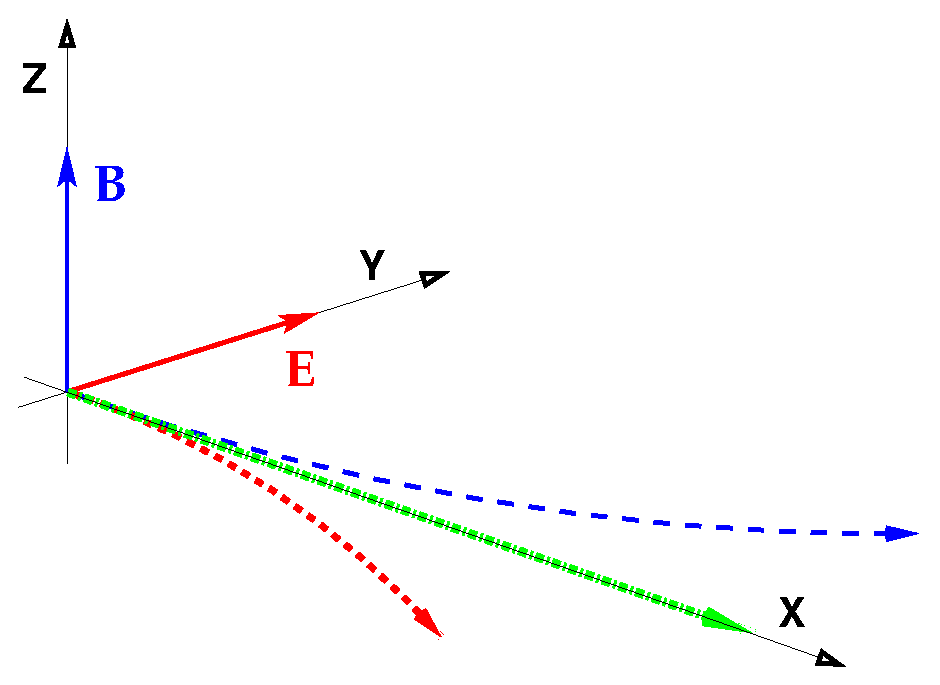
\includegraphics[width=.99\linewidth]{spinRotator.eps}
\end{minipage} 




\section*{ Numerical experiments }


\nin 1/ Set up a Wien filter in zgoubi with length  $ L=0.5$\,m, and $ B$ and $E$ such to (i)~ensure straight trajectory,
(ii)~ensure 30$^o$  spin Z-rotation.

FIT can be used. 

Compare with theory.

~

\nin 2/  Check the effect of step size on the accuracy on spin rotation value: 

\medskip

2.a - Using REBELOTE, get a scan of $ \theta_Z $  for $ \Delta s$ varied from  .01\,cm to 10\,cm in 100 steps. 

Plot  $\theta_Z$ versus $ \Delta s $  (can use gnuplot to plot data read from zgoubi.fai).

\medskip

2.b - Let's do it differently, namely, check the effect of step size on E and B values instead:

 Add FIT prior to REBELOTE, so to constrain  $ \theta_Z $ to its expected 30$^o$ value.
The variables in the FIT are  E and B.

Plot  E and B versus $ \Delta s $. 


~

\nin 3/ Align three 30$^o$  Wien filter rotators to get 90$^o$  spin rotation.  Make sure the spin rotation amounts to the expected value.

Compute the spin transport matrix.


~

   \nin 3/ 
   Add fringe-fields, re-do a FIT on E and B for straight trajectory and $\theta_Z = 30^o$ spin rotation.

   Compare the new E and B values with the hard-edge case. 



\end{document}
